\documentclass[11pt]{article}
\usepackage[a4paper,margin=2.2cm]{geometry}
\usepackage{amsmath,amssymb,booktabs,graphicx,adjustbox}
\usepackage{natbib}
\usepackage[hidelinks]{hyperref}
\usepackage{placeins}
\usepackage{microtype}
\usepackage{titlesec}
\titlespacing*{\section}{0pt}{9pt plus 2pt minus 1pt}{4pt}
\titlespacing*{\subsection}{0pt}{7pt plus 2pt minus 1pt}{3pt}
\setlength{\bibsep}{1pt}
\setlength{\parskip}{3pt}
\setlength{\parindent}{1em}
\setlength{\textfloatsep}{10pt}
\setlength{\floatsep}{8pt}
\setlength{\intextsep}{8pt}
\renewcommand{\topfraction}{.95}
\renewcommand{\bottomfraction}{.95}
\renewcommand{\textfraction}{.05}
\renewcommand{\floatpagefraction}{.8}
% Generated numeric claims; provenance in provenance.json.
\newcommand{\fitCoefficient}{0.377}
\newcommand{\referenceCoefficient}{0.37}
\newcommand{\toyThreshold}{0.90}
\newcommand{\languageCap}{2}
\newcommand{\realWidth}{896}
\newcommand{\modelLayers}{24}
\newcommand{\kvPplFull}{8.57}
\newcommand{\kvPplMerged}{172904}
\newcommand{\kvPplDelta}{0.29}
\newcommand{\kvContext}{1.50}
\newcommand{\neuronCount}{116}
\newcommand{\crossReduction}{2.15}
\newcommand{\retentionLoss}{37.9}
\newcommand{\easyRecovery}{0.597}
\newcommand{\priorEasy}{0.124}
\newcommand{\surpriseLow}{3.13}
\newcommand{\surpriseHigh}{7.57}
\newcommand{\exitSaving}{6.1}
\newcommand{\exitEasy}{21.08}
\newcommand{\exitHard}{23.68}
\newcommand{\exitTokens}{1024}
\newcommand{\wmBits}{16}
\newcommand{\wmAlpha}{0.01}
\newcommand{\wmResidual}{0.9194}
\newcommand{\wmLogits}{0.5684}
\newcommand{\wmKL}{0.00035}
\newcommand{\wmAgreement}{1.0000}
\newcommand{\maxTrainedStreams}{32}
\newcommand{\imageCap}{4}
\newcommand{\rankPlateau}{6}
\newcommand{\rankFull}{14}
\newcommand{\languageThresholdPct}{80}
\newcommand{\retentionEasyExample}{0.698}
\newcommand{\retentionMiddleExample}{2.154}
\newcommand{\retentionExampleK}{4}
\newcommand{\fullTrainCap}{1}
\newcommand{\fullTrainAccuracy}{0.246}
\newcommand{\fullHeldoutCap}{2}
\newcommand{\fullHeldoutAccuracy}{0.207}
\newcommand{\selectiveTrainEasy}{0.686}
\newcommand{\selectiveTrainCutLow}{2.81}
\newcommand{\selectiveTrainCutHigh}{7.17}
\newcommand{\selectiveHeldoutEasy}{0.618}
\newcommand{\selectiveHeldoutCutLow}{3.10}
\newcommand{\selectiveHeldoutCutHigh}{7.79}
\newcommand{\languageCapMin}{1}
\newcommand{\languageCapMax}{2}
\newcommand{\retentionTwoMin}{76.8}
\newcommand{\retentionTwoMax}{87.0}
\newcommand{\retentionTwoMean}{81.2}
\newcommand{\retentionEightMin}{39.6}
\newcommand{\retentionEightMax}{51.2}
\newcommand{\retentionEightMean}{45.0}
\newcommand{\fullTrainRetentionTwo}{76.8}
\newcommand{\fullHeldoutRetentionTwo}{87.0}
\newcommand{\selectiveTrainCap}{1}
\newcommand{\selectiveTrainRetentionTwo}{77.9}
\newcommand{\selectiveHeldoutCap}{2}
\newcommand{\selectiveHeldoutRetentionTwo}{83.3}
\newcommand{\heldAccuracyEasyOne}{61.8}
\newcommand{\heldAccuracyMiddleOne}{1.0}
\newcommand{\heldAccuracyHardOne}{0.0}
\newcommand{\heldEasyRetentionOne}{100.0}
\newcommand{\heldAccuracyEasyTwo}{50.0}
\newcommand{\heldAccuracyMiddleTwo}{2.6}
\newcommand{\heldAccuracyHardTwo}{0.0}
\newcommand{\heldEasyRetentionTwo}{80.9}
\newcommand{\heldAccuracyEasyFour}{40.6}
\newcommand{\heldAccuracyMiddleFour}{3.3}
\newcommand{\heldAccuracyHardFour}{0.0}
\newcommand{\heldEasyRetentionFour}{65.7}
\newcommand{\heldAccuracyEasyEight}{25.1}
\newcommand{\heldAccuracyMiddleEight}{3.0}
\newcommand{\heldAccuracyHardEight}{0.0}
\newcommand{\heldEasyRetentionEight}{40.6}
\newcommand{\heldoutBatches}{32}
\newif\iflanguageHeldout
\languageHeldouttrue
\newif\ifsurpriseHeldout
\surpriseHeldouttrue
\newcommand{\languageGrid}{1,2,4,6,8}

\title{Engineered CDMA Superposition in Pretrained Transformers:\\Nonlinear Readout Failures, Capacity Limits,\\and Per-Token Surprise}
\author{Jose Joaqu\'in Vargas Altalaguerri\\Independent Researcher\\\texttt{jvargas8@xtec.cat}}
\date{November 2026}
\begin{document}
\maketitle
\begin{abstract}
Sign-coded superposition can carry recoverable signals through transformer activations without providing independent computation on those signals. We examine this distinction across five application-level readouts in Qwen2.5-0.5B: normalized unembedding, attention over merged caches, multiplexed MLP probing, multi-behavior steering, and parallel output prediction. None of the tested untrained decoders gives reliable independent recovery. For example, selective CDMA cache merging increases perplexity from \kvPplFull{} to \kvPplMerged{}, whereas matched eviction increases it by only \kvPplDelta{}. An exploratory width-to-symbol-information fit describes trained toy transformers, but causal-language $K_{\rm cap}^{\languageThresholdPct}$ ranges from \languageCapMin{} to \languageCapMax{} across evaluation samples: the largest evaluated $K$ retaining at least \languageThresholdPct\% of the same multistream-adapted checkpoint's $K=1$ accuracy, not intrinsic capacity. Threshold crossings are fragile; accuracy declines monotonically with stream count. Held-out target-token surprise remains descriptively associated with absolute accuracy under superposition; an additional oracle early-exit probe saves only \exitSaving\% of layer evaluations. Modality and binding-code controls do not provide a general remedy. A paired residual-stream watermark remains recoverable at KL divergence \wmKL{}, providing a positive control for transport rather than parallel reasoning. These findings support a task-dependent bottleneck, not an impossibility theorem about superposition or nonlinear networks.
\end{abstract}

\section{Introduction}
A compact activation can retain a signal that the rest of a model cannot use as an independently addressable computation. This distinction matters whenever engineered superposition is proposed as a shortcut to batching: recovering a sign from an activation does not establish that the model processed its associated task. Our central empirical claim is that the useful superposition in these experiments lives in a linear sensing channel, or in a decoder explicitly trained for multiplexing. Each tested untrained nonlinear readout fails to turn that channel into reliable independent computation.

We develop the scientific results previously confined to the appendices of \citet{previous}. The contribution is a controlled map of failures, their trained positive controls, and a descriptive association between target-token surprise and absolute accuracy under superposition. We do not introduce multiple-input multiple-output neural computation, already studied by \citet{menet2023}, nor claim that transformers cannot perform naturally composed tasks \citep{xiong2024}. ``Failure at every readout'' refers to the probes and operating points reported here, not every possible detector, model, or nonlinearity.

The working explanation is that task-dependent processing demand, denoted $D_{\rm task}$, matters more than geometric separability alone. The causal-language experiments are consistent with this explanation, but do not identify it uniquely: optimization, adaptation budget, and the objective also differ from the toy setting. The within-sample association is heterogeneous: low-surprise targets have higher absolute accuracy under superposition, but surprise is computed retrospectively from the same predictions and is not a pre-answer routing signal.

\section{The linear/nonlinear channel view}
Let $h\in\mathbb R^d$ be a residual vector, $C\in\{-1,+1\}^{d\times B}$ a sign-code matrix, and $b\in\{-1,+1\}^B$ a payload. A normalized additive signal is
\begin{equation}
 h'=h+\delta,\qquad \delta=\alpha\lVert h\rVert_2\frac{Cb}{\lVert Cb\rVert_2},\qquad
 \widehat b=\operatorname{sign}\!\left(C^\top(h'-h)\right).
 \label{eq:watermark}
\end{equation}
The implementation scales the columns of $C$ by $d^{-1/2}$, which cancels in the normalized injection. For task multiplexing, the analogous construction binds each stream $x_k$ coordinatewise:
\begin{equation}
 z=\sum_{k=1}^K c_k\odot E(x_k),\qquad
 \widehat x_k=G\!\left(c_k\odot F(z)\right).
 \label{eq:multiplex}
\end{equation}
Here $E$ is an embedding, $F$ the shared computation, and $G$ the readout. A linear map transports additive components exactly, but need not preserve code orthogonality or signal-to-noise ratio. Training can adapt $E,F,G$ to their binding scheme.

For a differentiable nonlinear map $f$, local transport is instead
\begin{equation}
 f(h+\delta)-f(h)=J_f(h)\delta+\mathcal O(\lVert\delta\rVert_2^2).
\end{equation}
The Jacobian depends on the operating point; a fixed correlator designed for $C$ need not match $J_f(h)C$. Attention additionally changes the routing weights of the mixture. Neither observation proves information destruction. In particular, the unembedding matrix itself is linear: ``logit barrier'' below includes the intervening stack, final RMS normalization, and a restricted detector, not a nonlinear matrix multiplication.

We use $D_{\rm task}$ as a conceptual demand on nonlinear processing. The heuristic $K D_{\rm task}\lesssim C_{\rm nl}(d)$ motivates the experiments; neither quantity is independently measured. The toy relation to $\log_2 V$ is an empirical fit, not a general channel-capacity theorem or a bound on inference speed.

\section{Experimental setup}
The pretrained-model experiments use Qwen2.5-0.5B. Its recorded width is $d=\realWidth$ and depth is \modelLayers{} layers. The real-language and selective-multiplexing probes adapt this checkpoint on WikiText; other probes test fixed pretrained weights. The toy models use synthetic sequence reversal or masked token reconstruction, with geometry and training settings stored alongside their results. These objectives must not be conflated with autoregressive language modeling.

Accuracy is exact target-token agreement, perplexity is exponentiated mean negative log likelihood, and watermark quality is bit agreement. Output fidelity is $D_{\rm KL}(p_{\rm clean}\Vert p_{\rm marked})$ and greedy-token agreement. Raw, relative, and chance-subtracted capacity criteria differ:
\begin{align}
 K_{\rm abs}&=\max\{K:A(K)\geq\tau_{\rm abs}\},\\
 K_{\rm rel}&=\max\{K:A(K)/A(1)\geq\tau_{\rm rel}\},\\
 K_{\rm signal}&=\max\{K:[A(K)-q]/[A(1)-q]\geq\tau_{\rm rel}\},
 \label{eq:capacity}
\end{align}
where $q$ is the chance baseline. The toy absolute threshold is \toyThreshold; the relative-threshold definition is encoded in the producer's \texttt{rel80}/\texttt{signal80} fields. Capacity is the largest qualifying \emph{tested} point. At the sweep endpoint it is a lower bound, and it is not meaningful if the single-stream signal is negligible.

All reported measurements are regenerated from frozen JSON. Watermark sample counts are not stored in that JSON; its producer specifies the prompt/position protocol rather than the smaller prompt count in the earlier manuscript. Positions from the same prompt are correlated; aggregate results do not support independent-sample confidence intervals. Clean and marked activations/logits are subtracted exactly, position by position. Divergent continuations also change context, so later differences are not pure local perturbations.

\section{Five nonlinear readout failures}
\subsection{Normalized unembedding and logits}
Table~\ref{tab:logits} contains every recorded amplitude and payload size, including the random-bit control. For the smallest payload and amplitude, residual recovery is \wmResidual{} while the transported-code logit detector reaches \wmLogits{}. The latter is weakly above nominal chance, so ``at chance'' would overstate the result without a valid uncertainty estimate. Larger amplitudes strongly perturb output without producing high-fidelity logit recovery.

The detector correlates paired logit differences with $WC$, where $W$ is the unembedding matrix. It omits the exact final-normalization Jacobian and does not fit an inverse or nonlinear decoder. Thus the result rejects this simple detector as a useful readout; it does not show that logits contain no recoverable information. Access to paired logits also exceeds ordinary text-only access.
% Generated by make_tables.py; do not edit.
\begin{table}[!htbp]
\centering\footnotesize\setlength{\tabcolsep}{3.3pt}
\caption{Paired watermark readouts: every recorded payload size and amplitude.}\label{tab:logits}
\begin{adjustbox}{max width=\linewidth}
\begin{tabular}{lrrrrrr}
\toprule
$B$ & $\alpha$ & Residual & Logits & Control & KL & Agreement \\
\midrule
16 & 0.01 & 0.9194 & 0.5684 & 0.5020 & 0.00035 & 1.0000 \\
16 & 0.02 & 0.9170 & 0.5581 & 0.5034 & 0.06077 & 0.9766 \\
16 & 0.05 & 0.8774 & 0.5488 & 0.4980 & 1.18703 & 0.8281 \\
16 & 0.1 & 0.8262 & 0.5620 & 0.4966 & 2.45799 & 0.6484 \\
16 & 0.2 & 0.7944 & 0.5386 & 0.5039 & 3.95222 & 0.4141 \\
16 & 0.4 & 0.8569 & 0.5322 & 0.5020 & 5.92412 & 0.1484 \\
64 & 0.01 & 0.7717 & 0.5480 & 0.4966 & 0.00029 & 0.9922 \\
64 & 0.02 & 0.7704 & 0.5459 & 0.4987 & 0.00117 & 0.9922 \\
64 & 0.05 & 0.7308 & 0.5331 & 0.4957 & 1.64037 & 0.8203 \\
64 & 0.1 & 0.7002 & 0.5289 & 0.4958 & 3.57792 & 0.6094 \\
64 & 0.2 & 0.6914 & 0.5305 & 0.4939 & 3.90638 & 0.4375 \\
64 & 0.4 & 0.7450 & 0.5432 & 0.5028 & 5.10210 & 0.2734 \\
256 & 0.01 & 0.6435 & 0.5220 & 0.4977 & 0.00032 & 0.9922 \\
256 & 0.02 & 0.6385 & 0.5221 & 0.4981 & 0.43778 & 0.9609 \\
256 & 0.05 & 0.6361 & 0.5218 & 0.4973 & 0.73892 & 0.8984 \\
256 & 0.1 & 0.6268 & 0.5249 & 0.4977 & 1.48889 & 0.7969 \\
256 & 0.2 & 0.5987 & 0.5185 & 0.5001 & 4.44739 & 0.3906 \\
256 & 0.4 & 0.6246 & 0.5251 & 0.5013 & 5.47730 & 0.2188 \\
\bottomrule
\end{tabular}
\end{adjustbox}
\par\smallskip{\scriptsize Exact clean--marked subtraction; the logit detector projects onto transported codes, not an optimized decoder.}
\end{table}


\subsection{Attention softmax and selective KV merging}
The cache experiment selects low-surprise positions and compares CDMA merging, arithmetic-mean merging, eviction, and a random-position CDMA control at matched storage reduction. It preserves absolute positional indexing. Table~\ref{tab:kv} shows catastrophic CDMA merging, while eviction yields an effective-context multiplier of \kvContext{} at a perplexity increment of \kvPplDelta{}. Arithmetic averaging also substantially outperforms sign-coded merging. This isolates failure of the proposed cache representation rather than failure of all cache compression.
% Generated by make_tables.py; do not edit.
\begin{table}[!htbp]
\centering\footnotesize\setlength{\tabcolsep}{3.3pt}
\caption{Complete KV-cache comparison at the recorded compression setting.}\label{tab:kv}
\begin{adjustbox}{max width=\linewidth}
\begin{tabular}{lrrrr}
\toprule
Method & NLL & PPL & Removed fraction & $K_{\rm eff}$ \\
\midrule
FULL & 2.149 & 8.572 & 0.00000 & 1.000 \\
CDMA-MERGE-EASY & 12.060 & 172903.667 & 0.33301 & 1.499 \\
MEAN-MERGE-EASY & 2.271 & 9.692 & 0.33301 & 1.499 \\
EVICT-EASY & 2.181 & 8.858 & 0.33301 & 1.499 \\
CDMA-MERGE-RANDOM & 12.320 & 224130.095 & 0.33301 & 1.499 \\
\bottomrule
\end{tabular}
\end{adjustbox}
\par\smallskip{\scriptsize $K_{\rm eff}$ denotes effective context per retained slot, not the number of CDMA streams. No sweep was recorded.}
\end{table}

\begin{figure}[!htbp]\centering
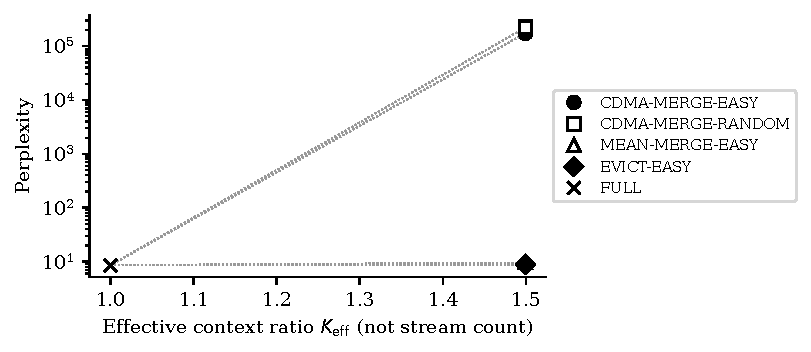
\includegraphics[width=.70\linewidth]{figures/kv_merge.pdf}
\caption{KV perplexity versus effective context ratio. Only the full-cache baseline and one compressed operating point exist; dotted connectors are not measured curves. The horizontal variable is not CDMA stream count.}\label{fig:kv}
\end{figure}

\subsection{MLP nonlinearity and ``neurosurgery''}
A targeted set of \neuronCount{} MLP neurons removes the measured concept response, but also damages general perplexity (Table~\ref{tab:mlp}). Unrelated accuracy is insufficient to certify capability preservation: the narrow control remains intact while fluency deteriorates. Random ablations of the same size are markedly less destructive to perplexity. The multiplexed concept scan also fails to reproduce its serial maps (Table~\ref{tab:mlp_maps}). These are application-level failures, not isolated causal measurements of the activation function.
% Generated by make_tables.py; do not edit.
\begin{table}[!htbp]
\centering\footnotesize\setlength{\tabcolsep}{3.3pt}
\caption{MLP ablation: targeted versus matched-size random control.}\label{tab:mlp}
\begin{adjustbox}{max width=\linewidth}
\begin{tabular}{lrrrrrrr}
\toprule
Fraction (\%) & Neurons & Target acc. & Other acc. & Target PPL & Random acc. & Other acc. & Random PPL \\
\midrule
Baseline & -- & 0.400 & 1.000 & 12.180 & -- & -- & -- \\
0.1 & 116 & 0.000 & 1.000 & 18.290 & 0.362 & 1.000 & 12.240 \\
0.5 & 583 & 0.000 & 1.000 & 24.230 & 0.476 & 1.000 & 12.370 \\
1.0 & 1167 & 0.000 & 1.000 & 28.770 & 0.505 & 1.000 & 12.770 \\
2.0 & 2334 & 0.000 & 1.000 & 34.700 & 0.514 & 1.000 & 13.170 \\
5.0 & 5836 & 0.000 & 1.000 & 44.560 & 0.448 & 1.000 & 15.730 \\
\bottomrule
\end{tabular}
\end{adjustbox}
\end{table}

% Generated by make_tables.py; do not edit.
\begin{table}[!htbp]
\centering\footnotesize\setlength{\tabcolsep}{3.3pt}
\caption{Multiplexed versus serial neuron maps, by concept.}\label{tab:mlp_maps}
\begin{adjustbox}{max width=\linewidth}
\begin{tabular}{lrr}
\toprule
Concept & Top-list overlap & Cosine \\
\midrule
capital & 0.260 & -0.196 \\
chemistry & 0.340 & -0.127 \\
continent & 0.240 & -0.162 \\
antonym & 0.360 & -0.155 \\
Mean & 0.300 & -0.160 \\
\bottomrule
\end{tabular}
\end{adjustbox}
\end{table}


\subsection{Downstream stack and eigen-steering}
Orthogonalizing behavior vectors reduces mean off-target coupling by only \crossReduction\%, while reducing mean on-target retention by \retentionLoss\% relative to naive addition. The previous shorthand ``halves retention'' is not numerically exact. Table~\ref{tab:steering} reports every behavior, single-vector baseline, simultaneous condition, and random control. Ratios may be negative or exceed unity, so their mean must not be interpreted as a bounded success probability. Better input geometry does not ensure independent downstream behavioral control.
% Generated by make_tables.py; do not edit.
\begin{table}[!htbp]
\centering\footnotesize\setlength{\tabcolsep}{3.3pt}
\caption{All steering behaviors and controls; effects are changes from baseline.}\label{tab:steering}
\begin{adjustbox}{max width=\linewidth}
\begin{tabular}{lrrrrrr}
\toprule
Behavior & Single & Naive & Ortho. & Random & $R_{\rm naive}$ & $R_{\rm ortho}$ \\
\midrule
sentiment & 0.067 & -0.067 & -0.067 & -0.067 & -1.000 & -1.000 \\
language & 1.127 & 1.013 & 1.073 & 0.000 & 0.899 & 0.953 \\
verbosity & 0.130 & 0.230 & 0.137 & -0.970 & 1.769 & 1.051 \\
topic\_food & 0.400 & 0.033 & 0.033 & 0.000 & 0.083 & 0.083 \\
Mean retention & -- & -- & -- & -- & 0.438 & 0.272 \\
Mean cross-coupling & -- & 0.387 & 0.379 & -- & -- & -- \\
\bottomrule
\end{tabular}
\end{adjustbox}
\par\smallskip{\scriptsize Retention is a ratio to the single-behavior effect: negative values and values above unity are possible.}
\end{table}


\subsection{Output and parallel multiplexing}
Table~\ref{tab:multiplex} compares extracted and random directions at every recorded stream count and amplitude. Hidden-state correlation can remain high while the original per-stream output targets do not survive. This is a transport--computation dissociation, not evidence of practical parallel generation. The additional sensing and depth controls are retained in Tables~\ref{tab:viability}--\ref{tab:depth}; the stored depth-break statistic has a pre-injection numerical artifact and is not used as a quantitative depth limit.
% Generated by make_tables.py; do not edit.
\begin{table}[!htbp]
\centering\footnotesize\setlength{\tabcolsep}{3.3pt}
\caption{Output multiplexing: all amplitudes, stream counts, and both code controls.}\label{tab:multiplex}
\begin{adjustbox}{max width=\linewidth}
\begin{tabular}{lrrrrrrrrr}
\toprule
$\alpha$ & $K$ & $h_E$ & $n_E$ & $s_E$ & $t_E$ & $h_R$ & $n_R$ & $s_R$ & $t_R$ \\
\midrule
0.050 & 2 & 1.000 & 1.000 & 0.000 & 1.000 & 1.000 & 0.052 & 0.000 & 1.000 \\
0.050 & 4 & 1.000 & 1.000 & 0.000 & 0.750 & 1.000 & 0.103 & 0.000 & 1.000 \\
0.050 & 8 & 1.000 & 1.000 & 0.000 & 0.880 & 1.000 & 0.202 & 0.000 & 1.000 \\
0.050 & 16 & 1.000 & 1.000 & 0.000 & 0.940 & 1.000 & 0.558 & 0.000 & 0.940 \\
0.050 & 32 & 0.938 & 1.000 & 0.000 & 0.940 & 1.000 & 0.547 & 0.000 & 1.000 \\
0.150 & 2 & 1.000 & 1.000 & 0.000 & 1.000 & 1.000 & 0.048 & 0.000 & 1.000 \\
0.150 & 4 & 1.000 & 1.000 & 0.000 & 1.000 & 1.000 & 0.230 & 0.000 & 1.000 \\
0.150 & 8 & 1.000 & 1.000 & 0.000 & 1.000 & 1.000 & 0.491 & 0.000 & 1.000 \\
0.150 & 16 & 1.000 & 1.000 & 0.000 & 0.940 & 0.875 & 0.651 & 0.000 & 1.000 \\
0.150 & 32 & 0.750 & 1.000 & 0.000 & 0.910 & 0.625 & 0.834 & 0.000 & 0.970 \\
0.300 & 2 & 1.000 & 1.000 & 0.000 & 1.000 & 1.000 & 0.312 & 0.000 & 1.000 \\
0.300 & 4 & 1.000 & 1.000 & 0.000 & 1.000 & 1.000 & 0.368 & 0.000 & 1.000 \\
0.300 & 8 & 1.000 & 1.000 & 0.000 & 1.000 & 1.000 & 0.456 & 0.000 & 1.000 \\
0.300 & 16 & 0.750 & 1.000 & 0.000 & 1.000 & 1.000 & 0.563 & 0.000 & 1.000 \\
0.300 & 32 & 0.813 & 1.000 & 0.031 & 0.940 & 0.937 & 0.669 & 0.000 & 0.940 \\
\bottomrule
\end{tabular}
\end{adjustbox}
\par\smallskip{\scriptsize $E/R$: extracted/random; $h$: hidden correlation; $n$: null ratio; $s$: logit survival; $t$: distinct-target fraction.}
\end{table}

\FloatBarrier

\section{Exploratory empirical capacity fit}
\subsection{Repaired toy configurations}
The repaired synthetic reversal cells yield an exploratory empirical capacity fit
\begin{equation}
 K_{\rm cap}\approx a\,\frac{d}{\log_2 V},\qquad a\simeq\referenceCoefficient.
 \label{eq:fit}
\end{equation}
The through-origin least-squares coefficient is \fitCoefficient; \referenceCoefficient{} is its truncated reference. Repaired cells replace matching original configurations, and the fit uses that substituted set, not an independent validation set (Table~\ref{tab:capacity}). This is not a capacity law: validation on configurations and seeds excluded from fitting has not been performed. Complete accuracy grids appear in Table~\ref{tab:toy_curves}.
% Generated by make_tables.py; do not edit.
\begin{table}[!htbp]
\centering\footnotesize\setlength{\tabcolsep}{3.3pt}
\caption{Every toy capacity cell, before and after targeted curriculum repairs.}\label{tab:capacity}
\begin{adjustbox}{max width=\linewidth}
\begin{tabular}{lrrrr}
\toprule
Run & $d$ & $V$ & $K_{\rm cap}$ & $K_{\rm cap}\log_2(V)/d$ \\
\midrule
Original & 64 & 16 & 0 & 0.000 \\
Original & 128 & 16 & 12 & 0.375 \\
Original & 256 & 16 & 24 & 0.375 \\
Original & 64 & 64 & 0 & 0.000 \\
Original & 128 & 64 & 4 & 0.188 \\
Original & 256 & 64 & 16 & 0.375 \\
Repair & 64 & 16 & 5 & 0.312 \\
Repair & 64 & 64 & 3 & 0.281 \\
Repair & 128 & 64 & 10 & 0.469 \\
\bottomrule
\end{tabular}
\end{adjustbox}
\par\smallskip{\scriptsize The fit uses repaired cells in place of their original counterparts. Original failures remain visible; repairs change the training curriculum/budget.}
\end{table}

\begin{figure}[!htbp]\centering
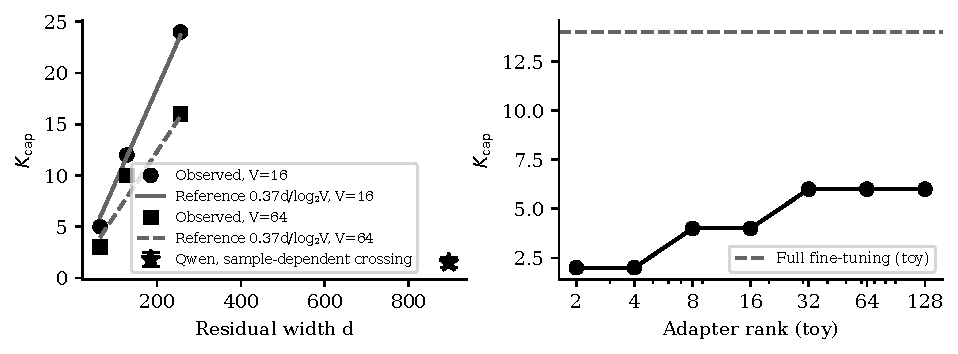
\includegraphics[width=.85\linewidth]{figures/capacity.pdf}
\caption{Left: repaired toy capacity and exploratory fit reference; the Qwen marker spans observed train/held-out threshold crossings on $K\in\{\languageGrid\}$, one checkpoint and one budget, retaining at least \languageThresholdPct\% of its $K=1$ accuracy, not an intrinsic capacity. Right: toy adapter-rank sweep and full-training control. No real-language vocabulary size is recorded in these JSON, so a numerical extrapolation to Qwen is not fabricated.}\label{fig:capacity}
\end{figure}

\subsection{LoRA, full fine-tuning, and rank}
The toy rank sweep plateaus at \rankPlateau{} streams against a full-control capacity of \rankFull{} (Table~\ref{tab:rank}). The adaptation-location ablation (Table~\ref{tab:hybrid}) shows that parameterization matters in the toy regime. We do not fit a logarithmic rank relation from this sparse grid.
% Generated by make_tables.py; do not edit.
\begin{table}[!htbp]
\centering\footnotesize\setlength{\tabcolsep}{3.3pt}
\caption{Complete adapter-rank sweep on the toy task.}\label{tab:rank}
\begin{adjustbox}{max width=\linewidth}
\begin{tabular}{lrrrrrrrrrrr}
\toprule
Rank & Trainable parameters & $K_{\rm cap}$ & $1$ & $2$ & $4$ & $6$ & $8$ & $10$ & $12$ & $14$ & $16$ \\
\midrule
2 & 15888 & 2 & 0.997 & 0.949 & 0.472 & 0.196 & 0.089 & 0.074 & 0.072 & 0.069 & 0.068 \\
4 & 29712 & 2 & 1.000 & 0.997 & 0.735 & 0.415 & 0.106 & 0.083 & 0.078 & 0.073 & 0.070 \\
8 & 57360 & 4 & 1.000 & 1.000 & 0.937 & 0.629 & 0.129 & 0.098 & 0.087 & 0.082 & 0.077 \\
16 & 112656 & 4 & 0.992 & 1.000 & 0.994 & 0.837 & 0.246 & 0.123 & 0.107 & 0.096 & 0.091 \\
32 & 223248 & 6 & 1.000 & 1.000 & 0.999 & 0.950 & 0.472 & 0.163 & 0.144 & 0.129 & 0.118 \\
64 & 444432 & 6 & 1.000 & 1.000 & 0.999 & 0.978 & 0.762 & 0.177 & 0.157 & 0.144 & 0.128 \\
128 & 886800 & 6 & 0.993 & 0.998 & 0.998 & 0.977 & 0.816 & 0.192 & 0.170 & 0.154 & 0.139 \\
Full & 613776 & 14 & -- & -- & -- & -- & -- & -- & -- & -- & -- \\
\bottomrule
\end{tabular}
\end{adjustbox}
\par\smallskip{\scriptsize Accuracy columns are indexed by stream count. The full-control JSON records capacity but not its curve.}
\end{table}

% Generated by make_tables.py; do not edit.
\begin{table}[!htbp]
\centering\footnotesize\setlength{\tabcolsep}{3.3pt}
\caption{Toy adaptation ablation, with complete accuracy curves.}\label{tab:hybrid}
\begin{adjustbox}{max width=\linewidth}
\begin{tabular}{lrrrrrrrrrr}
\toprule
Condition & $1$ & $2$ & $4$ & $6$ & $8$ & $10$ & $12$ & $14$ & $16$ & $K_{\rm cap}$ \\
\midrule
full & 1.000 & 1.000 & 1.000 & 1.000 & 1.000 & 0.995 & 0.978 & 0.935 & 0.844 & 14 \\
lora\_both & 1.000 & 1.000 & 0.987 & 0.777 & 0.192 & 0.123 & 0.108 & 0.099 & 0.093 & 4 \\
lora\_mlp & 0.999 & 0.998 & 0.704 & 0.254 & 0.080 & 0.070 & 0.066 & 0.066 & 0.065 & 2 \\
lora\_attn & 1.000 & 0.998 & 0.852 & 0.489 & 0.162 & 0.121 & 0.109 & 0.102 & 0.095 & 2 \\
frozen & 1.000 & 0.193 & 0.104 & 0.081 & 0.072 & 0.069 & 0.066 & 0.066 & 0.064 & 1 \\
\bottomrule
\end{tabular}
\end{adjustbox}
\end{table}


The original LoRA and full-fine-tuning curves are \emph{in-sample}: evaluation resamples training tokens. Their threshold crossing is not intrinsic capacity: $K_{\rm cap}^{\languageThresholdPct}$ is the largest evaluated $K$ retaining at least \languageThresholdPct\% of the $K=1$ accuracy of the same checkpoint trained with a multistream curriculum, not a separately adapted single-stream model. The full/initial LoRA grid is $K\in\{\languageGrid\}$; the selective LoRA evaluation omits the intermediate full-FT grid point. Each adaptation uses one checkpoint and one training budget.
\iflanguageHeldout
Table~\ref{tab:language} now includes independently evaluated WikiText validation tokens. Full fine-tuning gives new-train $K=1$ accuracy \fullTrainAccuracy{} and held-out accuracy \fullHeldoutAccuracy{}, with threshold crossings \fullTrainCap{} and \fullHeldoutCap{}, respectively.
\ifsurpriseHeldout
The selective LoRA run similarly crosses at \selectiveTrainCap{} on new train windows and \selectiveHeldoutCap{} held-out. Thus $K_{\rm cap}^{\languageThresholdPct}$ lies between \languageCapMin{} and \languageCapMax{} depending on evaluation sample, rather than establishing a fixed language limit. For example, full-FT train retention at $K=2$ is \fullTrainRetentionTwo\%, below the \languageThresholdPct\% cutoff; held-out retention is \fullHeldoutRetentionTwo\%. The threshold statistic is fragile near that cutoff. The robust pattern is monotonically declining absolute accuracy: $K=2$ retains \retentionTwoMin--\retentionTwoMax\% of $K=1$ accuracy, while $K=8$ retains \retentionEightMin--\retentionEightMax\% across the new train/held-out curves (mean \retentionEightMean\%, approximately half). These aggregate results do not supply uncertainty estimates or exclude optimization/budget effects.
\fi
\else
No held-out full-fine-tuning JSON is available; out-of-sample evidence is pending.
\fi
% Generated by make_tables.py; do not edit.
\begin{table}[!htbp]
\centering\footnotesize\setlength{\tabcolsep}{3.3pt}
\caption{Causal language modeling: original in-sample curves and train/held-out evaluation.}\label{tab:language}
\begin{adjustbox}{max width=\linewidth}
\begin{tabular}{lrrrrrr}
\toprule
Condition & $1$ & $2$ & $4$ & $6$ & $8$ & $K_{\rm cap}$ \\
\midrule
No adaptation / original train & 0.007 & 0.008 & 0.013 & 0.008 & 0.005 & -- \\
LoRA / original train & 0.219 & 0.198 & 0.144 & 0.115 & 0.088 & 2 \\
Full FT / original train & 0.244 & 0.215 & 0.159 & 0.135 & 0.113 & 2 \\
Full FT / new train & 0.246 & 0.189 & 0.157 & 0.131 & 0.109 & 1 \\
Full FT / held-out & 0.207 & 0.180 & 0.154 & 0.137 & 0.106 & 2 \\
LoRA selective / new train & 0.235 & 0.183 & 0.147 & -- & 0.093 & 1 \\
LoRA selective / held-out & 0.210 & 0.175 & 0.146 & -- & 0.094 & 2 \\
\bottomrule
\end{tabular}
\end{adjustbox}
\par\smallskip{\scriptsize Train rows are in-sample; held-out rows are out-of-sample. The denominator is K=1 accuracy of the same multistream-adapted checkpoint, not a separately adapted model. Capacity is a grid threshold crossing, not an intrinsic limit.}
\end{table}


\section{Descriptive association: target-token surprise and absolute accuracy}
For a target token $y_t$, define surprise under the adapted single-stream model as
\begin{equation}
 S_t=-\log p_1(y_t\mid x_{<t}),\qquad
 R_g(K)=\frac{A_g(K)}{A_g(1)},
\end{equation}
where $g$ indexes a fixed surprise tercile. The original numbers are \emph{in-sample}, computed on the training-token pool. Cut points are \surpriseLow{} and \surpriseHigh{} nats; easy-token accuracy at $K=1$ is \easyRecovery{}, versus constant-token-prior accuracy \priorEasy{}. The hard tercile has zero correct targets at $K=1$, so its relative retention is undefined. Table~\ref{tab:surprise} distinguishes these train results from any new split evaluation.
\ifsurpriseHeldout
The held-out association is now supported out of sample: easy-token accuracy at $K=1,2,4,8$ is \heldAccuracyEasyOne, \heldAccuracyEasyTwo, \heldAccuracyEasyFour, and \heldAccuracyEasyEight\%; easy-token retention is \heldEasyRetentionOne, \heldEasyRetentionTwo, \heldEasyRetentionFour, and \heldEasyRetentionEight\%. The middle group has low absolute accuracy and the hard group remains at zero even at $K=1$ (Table~\ref{tab:surprise}). Compared with new-train easy-token $K=1$ accuracy \selectiveTrainEasy{}, held-out accuracy is \selectiveHeldoutEasy{}; the qualitative association persists, while the overall threshold crossing changes as discussed above. Both splits use \heldoutBatches{} evaluation batches per stream count. Terciles are fitted independently within each evaluated split, not trained on one and transferred to the other; held-out cut points are \selectiveHeldoutCutLow{} and \selectiveHeldoutCutHigh{} nats. The shared-prediction coupling still applies.
\else
No held-out selective-recovery JSON is available; out-of-sample confirmation is pending. Regeneration adds separate train and held-out rows when supplied.
\fi
% Generated by make_tables.py; do not edit.
\begin{table}[!htbp]
\centering\footnotesize\setlength{\tabcolsep}{3.3pt}
\caption{Absolute target-token accuracy and relative retention by surprise tercile, with available split evaluation.}\label{tab:surprise}
\begin{adjustbox}{max width=\linewidth}
\begin{tabular}{lrrrrrrrr}
\toprule
Split & $K$ & Easy & Middle & Hard & All & $R_E$ & $R_M$ & $R_H$ \\
\midrule
Original train & 1 & 0.597 & 0.013 & 0.000 & 0.203 & 1.000 & 1.000 & -- \\
Original train & 2 & 0.506 & 0.018 & 0.000 & 0.175 & 0.848 & 1.385 & -- \\
Original train & 4 & 0.417 & 0.028 & 0.000 & 0.148 & 0.698 & 2.154 & -- \\
Original train & 8 & 0.265 & 0.024 & 0.000 & 0.096 & 0.444 & 1.846 & -- \\
Original train & Prior & 0.124 & 0.008 & 0.000 & 0.044 & -- & -- & -- \\
New train & 1 & 0.686 & 0.019 & 0.000 & 0.235 & 1.000 & 1.000 & -- \\
New train & 2 & 0.511 & 0.037 & 0.000 & 0.183 & 0.745 & 1.947 & -- \\
New train & 4 & 0.402 & 0.039 & 0.000 & 0.147 & 0.586 & 2.053 & -- \\
New train & 8 & 0.246 & 0.031 & 0.000 & 0.093 & 0.359 & 1.632 & -- \\
New train & Prior & 0.117 & 0.013 & 0.000 & 0.043 & -- & -- & -- \\
Held-out & 1 & 0.618 & 0.010 & 0.000 & 0.210 & 1.000 & 1.000 & -- \\
Held-out & 2 & 0.500 & 0.026 & 0.000 & 0.175 & 0.809 & 2.600 & -- \\
Held-out & 4 & 0.406 & 0.033 & 0.000 & 0.146 & 0.657 & 3.300 & -- \\
Held-out & 8 & 0.251 & 0.030 & 0.000 & 0.094 & 0.406 & 3.000 & -- \\
Held-out & Prior & 0.131 & 0.011 & 0.000 & 0.047 & -- & -- & -- \\
\bottomrule
\end{tabular}
\end{adjustbox}
\par\smallskip{\scriptsize Train rows are in-sample; held-out rows use validation tokens. Terciles are fitted independently within each split, not transferred from train. Zero-denominator retention is undefined (--); relative retention need not order the terciles.}
\end{table}

\begin{figure}[!htbp]\centering
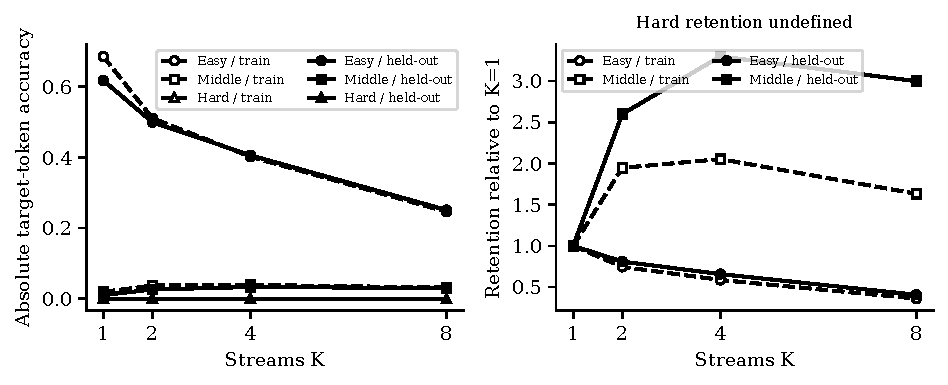
\includegraphics[width=.85\linewidth]{figures/surprise.pdf}
\caption{New train and held-out absolute accuracy and relative retention by target-token surprise tercile, with split-specific terciles. Relative retention does not order the groups; the middle-tercile ratio has a small denominator and hard-tercile retention is undefined.}\label{fig:surprise}
\end{figure}
Surprise and correctness are computed from the same single-stream predictions, so the association is descriptive and baseline enrichment is expected. The result concerns \emph{absolute} target-token accuracy under superposition; relative retention does not order the groups: at $K=\retentionExampleK$, $R_E=\retentionEasyExample$ whereas $R_M=\retentionMiddleExample$, with an unstable small middle-tercile denominator. Target-token surprise requires the answer and is not a predictor available before the response. No selective scheduler or throughput saving is established.

\paragraph{A negative early-exit control.}
The additional probe applies the final normalization and output head at each layer and finds the earliest layer after which all argmax predictions agree with the final one. Across \exitTokens{} positions, mean exits range from \exitEasy{} to \exitHard{} of \modelLayers{} layers, and the pooled layer-count saving is only \exitSaving\% (Table~\ref{tab:early_exit}). This is an oracle stable-exit statistic, not an executable stopping policy. It excludes head-evaluation overhead and does not measure latency. Its surprise is final-distribution top-prediction surprise, unlike the target-token surprise above. Therefore the result is consistent with limited depth redundancy, but not a direct test of the same surprise partition. Heterogeneity in recoverability does not automatically imply early computation can be skipped.
% Generated by make_tables.py; do not edit.
\begin{table}[!htbp]
\centering\footnotesize\setlength{\tabcolsep}{3.3pt}
\caption{Oracle stable-argmax early-exit probe (no trained exit heads).}\label{tab:early_exit}
\begin{adjustbox}{max width=\linewidth}
\begin{tabular}{lrrr}
\toprule
Group & Mean exit layer & Exit by half depth (\%) & Layer-count saving (\%) \\
\midrule
Easy & 21.08 & 0.00 & 12.20 \\
Middle & 22.85 & 0.00 & 4.80 \\
Hard & 23.68 & 0.00 & 1.30 \\
All & 22.54 & 0.00 & 6.10 \\
\bottomrule
\end{tabular}
\end{adjustbox}
\par\smallskip{\scriptsize Savings exclude exit-head cost and are not measured wall-clock or FLOP reductions; surprise differs from the target-token accuracy probe.}
\end{table}


\section{Modality and code design are not general levers}
The masked-reconstruction controls separate task and tokenizer effects from causal-language adaptation. Image capacity depends on vocabulary and setup; it is not a universal modality constant. With the larger recorded vocabulary, k-means and VQ-VAE image tokens have capacity \imageCap{}, whereas text and code remain signal-preserving to the extended sweep endpoint of \maxTrainedStreams{} streams. The latter is a lower bound, not an observed failure threshold. Figure~\ref{fig:modalities} distinguishes censored endpoints; Tables~\ref{tab:vision_kcap}--\ref{tab:code_kcap} retain every measured accuracy.
\begin{figure}[!htbp]\centering
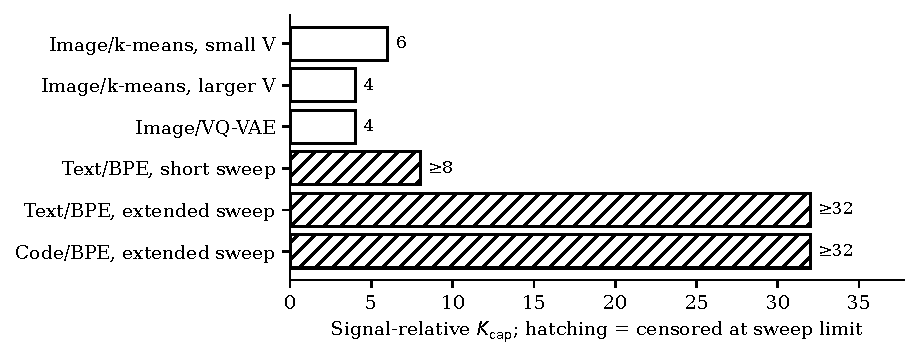
\includegraphics[width=.86\linewidth]{figures/modalities.pdf}
\caption{Signal-relative capacity across modality/tokenizer controls. Hatching denotes a sweep-limited lower bound. These masked toy objectives are not matched to causal language modeling.}\label{fig:modalities}
\end{figure}
Hadamard, random-sign, and highly correlated binding codes all preserve reconstruction through the tested endpoint under training (Table~\ref{tab:coded_vocab_kcap}). This refutes code orthogonality as a sufficient practical lever in this trained setting, not its relevance in every model. It is consistent with learned embeddings compensating for the code, but does not prove that mechanism. The results alone also do not identify image-token rank, correlation, or redundancy as the cause of its lower capacity.
% Generated by make_tables.py; do not edit.
\begin{table}[!htbp]
\centering\footnotesize\setlength{\tabcolsep}{3.3pt}
\caption{Modality / tokenizer comparison: vision\_kcap.}\label{tab:vision_kcap}
\begin{adjustbox}{max width=\linewidth}
\begin{tabular}{lrrrrrrrr}
\toprule
Condition / state & $1$ & $2$ & $3$ & $4$ & $6$ & $8$ & $K_{\rm cap}$ & Signal at single stream \\
\midrule
random / untrained & 0.0150 & 0.0150 & 0.0160 & 0.0160 & 0.0160 & 0.0160 & -- & -- \\
random / trained & 0.0150 & 0.0160 & 0.0150 & 0.0160 & 0.0160 & 0.0150 & 1 & -0.0006 \\
text / untrained & 0.0010 & 0.0350 & 0.0300 & 0.0310 & 0.0210 & 0.0190 & -- & -- \\
text / trained & 0.1950 & 0.1910 & 0.1920 & 0.1930 & 0.1930 & 0.1920 & 8 & 0.1794 \\
image / untrained & 0.0110 & 0.0130 & 0.0190 & 0.0160 & 0.0170 & 0.0150 & -- & -- \\
image / trained & 0.3450 & 0.3310 & 0.3260 & 0.3240 & 0.3000 & 0.2640 & 6 & 0.3294 \\
\bottomrule
\end{tabular}
\end{adjustbox}
\par\smallskip{\scriptsize Capacity is signal-relative. A capacity at the largest tested stream count is a lower bound; random controls have negligible signal and no meaningful capacity.}
\end{table}

% Generated by make_tables.py; do not edit.
\begin{table}[!htbp]
\centering\footnotesize\setlength{\tabcolsep}{3.3pt}
\caption{Modality / tokenizer comparison: vision\_kcap\_hardvocab.}\label{tab:vision_kcap_hardvocab}
\begin{adjustbox}{max width=\linewidth}
\begin{tabular}{lrrrrrrrr}
\toprule
Condition / state & $1$ & $2$ & $3$ & $4$ & $6$ & $8$ & $K_{\rm cap}$ & Signal at single stream \\
\midrule
random / trained & 0.0019 & 0.0019 & 0.0022 & 0.0020 & 0.0019 & 0.0022 & 1 & -0.0001 \\
text\_bpe / trained & 0.3723 & 0.3669 & 0.3650 & 0.3620 & 0.3600 & 0.3582 & 8 & 0.3703 \\
image / trained & 0.1996 & 0.1916 & 0.1732 & 0.1687 & 0.1465 & 0.1145 & 4 & 0.1976 \\
\bottomrule
\end{tabular}
\end{adjustbox}
\par\smallskip{\scriptsize Capacity is signal-relative. A capacity at the largest tested stream count is a lower bound; random controls have negligible signal and no meaningful capacity.}
\end{table}

% Generated by make_tables.py; do not edit.
\begin{table}[!htbp]
\centering\footnotesize\setlength{\tabcolsep}{3.3pt}
\caption{Modality / tokenizer comparison: vqvae\_kcap.}\label{tab:vqvae_kcap}
\begin{adjustbox}{max width=\linewidth}
\begin{tabular}{lrrrrrrrr}
\toprule
Condition / state & $1$ & $2$ & $3$ & $4$ & $6$ & $8$ & $K_{\rm cap}$ & Signal at single stream \\
\midrule
image\_vqvae / trained & 0.1011 & 0.1008 & 0.0928 & 0.0932 & 0.0787 & 0.0631 & 4 & 0.0991 \\
image\_kmeans / trained & 0.1996 & 0.1916 & 0.1732 & 0.1687 & 0.1465 & 0.1145 & 4 & 0.1976 \\
text\_bpe / trained & 0.3723 & 0.3669 & 0.3650 & 0.3620 & 0.3600 & 0.3582 & 8 & 0.3703 \\
random / trained & 0.0019 & 0.0019 & 0.0022 & 0.0020 & 0.0019 & 0.0022 & 1 & -0.0001 \\
\bottomrule
\end{tabular}
\end{adjustbox}
\par\smallskip{\scriptsize Capacity is signal-relative. A capacity at the largest tested stream count is a lower bound; random controls have negligible signal and no meaningful capacity.}
\end{table}

% Generated by make_tables.py; do not edit.
\begin{table}[!htbp]
\centering\footnotesize\setlength{\tabcolsep}{3.3pt}
\caption{Modality / tokenizer comparison: code\_kcap.}\label{tab:code_kcap}
\begin{adjustbox}{max width=\linewidth}
\begin{tabular}{lrrrrrrrrrr}
\toprule
Condition / state & $1$ & $2$ & $4$ & $8$ & $12$ & $16$ & $24$ & $32$ & $K_{\rm cap}$ & Signal at single stream \\
\midrule
random / trained & 0.0022 & 0.0023 & 0.0016 & 0.0020 & 0.0019 & 0.0020 & 0.0020 & 0.0020 & 1 & 0.0002 \\
text\_bpe / trained & 0.3571 & 0.3540 & 0.3637 & 0.3613 & 0.3556 & 0.3609 & 0.3567 & 0.3577 & 32 & 0.3551 \\
code / trained & 0.3185 & 0.3244 & 0.3244 & 0.3229 & 0.3236 & 0.3216 & 0.3249 & 0.3221 & 32 & 0.3165 \\
\bottomrule
\end{tabular}
\end{adjustbox}
\par\smallskip{\scriptsize Capacity is signal-relative. A capacity at the largest tested stream count is a lower bound; random controls have negligible signal and no meaningful capacity.}
\end{table}

% Generated by make_tables.py; do not edit.
\begin{table}[!htbp]
\centering\footnotesize\setlength{\tabcolsep}{3.3pt}
\caption{Modality / tokenizer comparison: coded\_vocab\_kcap.}\label{tab:coded_vocab_kcap}
\begin{adjustbox}{max width=\linewidth}
\begin{tabular}{lrrrrrrrr}
\toprule
Condition / state & $1$ & $2$ & $4$ & $8$ & $16$ & $32$ & $K_{\rm cap}$ & Coherence \\
\midrule
random\_pm1 / trained & 0.3562 & 0.3633 & 0.3534 & 0.3607 & 0.3597 & 0.3588 & 32 & 0.2656 \\
hadamard / trained & 0.3715 & 0.3623 & 0.3589 & 0.3529 & 0.3586 & 0.3584 & 32 & 0.0000 \\
correlated / trained & 0.3479 & 0.3636 & 0.3567 & 0.3573 & 0.3582 & 0.3586 & 32 & 0.9687 \\
\bottomrule
\end{tabular}
\end{adjustbox}
\par\smallskip{\scriptsize Capacity is signal-relative. A capacity at the largest tested stream count is a lower bound; random controls have negligible signal and no meaningful capacity.}
\end{table}


\section{Positive control: the residual-stream watermark survives}
At $B=\wmBits$ and $\alpha=\wmAlpha$, paired residual recovery is \wmResidual{}, with KL \wmKL{} and greedy-token agreement \wmAgreement{} (Table~\ref{tab:logits}). Figure~\ref{fig:watermark} contrasts this with the weak logit detector. The small but nonzero divergence should not be called exact invariance. This positive control supports recoverable low-amplitude activation transport, not a robust text watermark or independent task computation. The companion \emph{Paper A: Activation-side session tagging for LLM audit logs} \citep{companion}, by the same author in the same repository, treats the audit-log system; it has no assigned DOI. Its scale study (Qwen2.5-0.5B/1.5B/7B, 128 sessions of 128 greedy tokens) confirms the linear-channel picture in both directions: the tag is recovered only by paired replay against the logged residual, blind decoding with a static calibration is at chance, a tag added directly at the read layer decodes perfectly (the residual response to a small perturbation is close to identity, so the mark proves transport, not computation), and the same $\alpha$ that leaves next-token agreement at \wmAgreement{} here changes most 128-token continuations on the larger models. The present exact paired-subtraction experiment must not be equated with a deployable single-log verifier.
\begin{figure}[!htbp]\centering
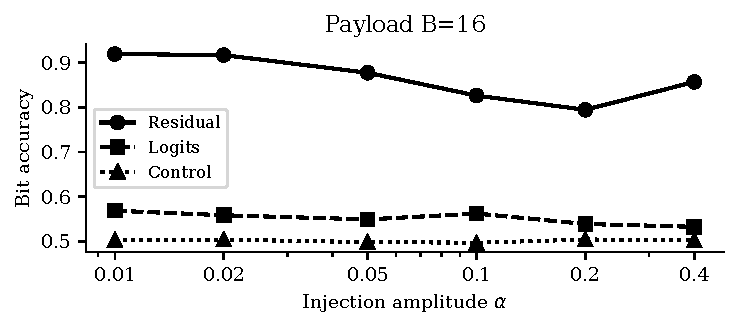
\includegraphics[width=.66\linewidth]{figures/watermark.pdf}
\caption{Residual, logit, and random-control bit accuracy for the smallest recorded payload, over all injection amplitudes.}\label{fig:watermark}
\end{figure}
Trained MLP and transformer controls (Tables~\ref{tab:trained_mlp} and \ref{tab:trained_transformer}) demonstrate that nonlinear networks can learn multiplexing. They constrain the failure claim to untrained engineered readouts and their objectives.

\section{Related work and honest novelty}
\citet{elhage2022} study learned feature superposition, not imposed codes. \citet{menet2023} train multiple-input multiple-output networks for superposed computation. Natural in-context task composition \citep{xiong2024} differs from sign-bound activation addition. ParScale \citep{chen2025} aggregates separate learned parallel passes, not one unmodified residual mixture.

\citet{borobia2026} study leverage dispersion and near-floor geometry in trained overcomplete codes, not a theorem about the nonlinear application failures tested here.

EntropyCache \citep{cheong2026} uses decoded-token entropy for diffusion-model cache refresh, not causal-model multiplexing. Text watermarking \citep{kirchenbauer2023} changes token selection, unlike paired activation sensing. BitNet \citep{wang2023} and Mamba \citep{gu2023} change weight computation or sequence architecture, without establishing free capacity for CDMA streams. Our contribution is the combined negative evidence and its surprise-stratified qualification, not a new multiplexing mechanism or universal information-theoretic law.

\section{Limitations}
All real-LLM results concern one small checkpoint, without cross-family or larger-scale replication. The original adaptation and surprise accuracies measure within-corpus recovery; the new validation-token evaluations provide out-of-sample evidence for these trained runs, not independent-seed or cross-model replication. Sample sizes are small and correlated, seeds are not comprehensively replicated, and rounded aggregate JSON does not support reliable uncertainty estimates. Behavioral scores are narrow. The logit probe tests a restricted correlator, not optimal or text-only decoding, and the application probes do not causally isolate individual nonlinear operators.

The exploratory capacity fit comes from toy reversal with replacement training configurations, without validation on unseen configurations or seeds. Masked modality tasks, causal language modeling, and MLP sign recovery use different objectives and thresholds. Endpoint capacities are censored. Matching in-sample language threshold crossings under the tested budgets do not establish an intrinsic $D_{\rm task}$ limit. Surprise is partly tied to baseline correctness, and the early-exit statistic is retrospective. No scheduler, wall-clock acceleration, or general impossibility result follows from these experiments.

\section*{Changes from version 1}
We correct arXiv:2605.01192 and its earlier floor-theorem attribution, omit the unsupported real-language overprediction, call the toy relation exploratory, and report original in-sample and new held-out evidence separately, including the evaluation-dependent threshold crossing. The readout failures are not impossibility results.

\section*{Reproducibility}
Code and frozen results: \url{https://github.com/ttzrs/neural-cdma}. The previous manuscript is DOI \href{https://doi.org/10.5281/zenodo.20570543}{10.5281/zenodo.20570543}, not a DOI for this paper. From \texttt{papers/channel/}, run \texttt{bash build.sh}; no GPU or weights are required. \texttt{tables/provenance.json} records source hashes and numeric-macro derivations.

{\footnotesize\raggedright
Readouts: \texttt{watermark\_provenance.py}, \texttt{kv\_selective.py}, \texttt{cdma\_neurosurgery.py}, \texttt{eigen\_steering.py}, \texttt{multithread.py}.\par
Capacity: \texttt{capacity\_law.py}, \texttt{capacity\_fix.py}, \texttt{rank\_sweep.py}, \texttt{hybrid\_multiplex.py}, \texttt{validate\_llm*.py}, \texttt{validate\_llm\_full\_heldout.py}.\par
Surprise: \texttt{prototype\_selective.py}, \texttt{prototype\_selective\_heldout.py}, \texttt{early\_exit\_surprise.py}.\par
Modality: \texttt{vision\_kcap*.py}, \texttt{vqvae\_kcap.py}, \texttt{code\_kcap.py}, \texttt{coded\_vocab\_kcap.py}.\par
Controls: \texttt{train\_superposition.py}, \texttt{train\_transformer\_superposition.py}, \texttt{viability.py}, \texttt{profile\_depth.py}.\par}
Rebuilding regenerates presentation, not experiments.

\FloatBarrier
\appendix
\section{Complete supporting controls}
These tables retain toy accuracy grids, trained sign-accuracy controls, sensing results, and depth summaries. Raw regression errors and depth arrays remain in the hashed JSON; the break statistic is not used as a usable-depth claim.
% Generated by make_tables.py; do not edit.
\begin{table}[!htbp]
\centering\footnotesize\setlength{\tabcolsep}{3.3pt}
\caption{Complete toy accuracy curves (missing grid points are not interpolated).}\label{tab:toy_curves}
\begin{adjustbox}{max width=\linewidth}
\begin{tabular}{lrrrrrrrrrrrrrrr}
\toprule
Condition & $1$ & $2$ & $3$ & $4$ & $5$ & $6$ & $8$ & $10$ & $12$ & $16$ & $20$ & $24$ & $28$ & $32$ & $K_{\rm cap}$ \\
\midrule
Original d=64,V=16 & 0.271 & 0.278 & -- & 0.249 & -- & 0.218 & 0.198 & -- & 0.162 & 0.137 & -- & -- & -- & -- & 0 \\
Original d=128,V=16 & 1.000 & 1.000 & -- & 1.000 & -- & 1.000 & 0.996 & -- & 0.935 & 0.804 & 0.655 & 0.474 & 0.299 & 0.219 & 12 \\
Original d=256,V=16 & 1.000 & 1.000 & -- & 1.000 & -- & 1.000 & 1.000 & -- & 1.000 & 0.999 & 0.989 & 0.958 & 0.897 & 0.793 & 24 \\
Original d=64,V=64 & 0.187 & 0.176 & -- & 0.129 & -- & 0.101 & 0.084 & -- & 0.063 & 0.052 & -- & -- & -- & -- & 0 \\
Original d=128,V=64 & 0.974 & 0.974 & -- & 0.941 & -- & 0.806 & 0.626 & -- & 0.274 & 0.154 & 0.107 & 0.086 & 0.070 & 0.063 & 4 \\
Original d=256,V=64 & 1.000 & 1.000 & -- & 1.000 & -- & 1.000 & 0.999 & -- & 0.983 & 0.923 & 0.830 & 0.729 & 0.633 & 0.544 & 16 \\
Repair d=64,V=16 & 1.000 & 1.000 & 0.997 & 0.990 & 0.954 & 0.873 & 0.614 & 0.345 & -- & -- & -- & -- & -- & -- & 5 \\
Repair d=64,V=64 & 0.994 & 0.997 & 0.974 & 0.894 & 0.757 & 0.548 & -- & -- & -- & -- & -- & -- & -- & -- & 3 \\
Repair d=128,V=64 & 1.000 & 1.000 & -- & 1.000 & -- & 0.997 & 0.972 & 0.900 & 0.773 & -- & -- & -- & -- & -- & 10 \\
\bottomrule
\end{tabular}
\end{adjustbox}
\end{table}

% Generated by make_tables.py; do not edit.
\begin{table}[!htbp]
\centering\footnotesize\setlength{\tabcolsep}{3.3pt}
\caption{Trained-transformer positive control: token-reversal accuracy.}\label{tab:trained_transformer}
\begin{adjustbox}{max width=\linewidth}
\begin{tabular}{lrrrrrrr}
\toprule
Condition & $1$ & $2$ & $3$ & $4$ & $6$ & $8$ & $K_{\rm cap}$ \\
\midrule
Untrained & 0.057 & 0.061 & 0.064 & 0.062 & 0.062 & 0.065 & -- \\
Trained & 1.000 & 0.999 & 0.998 & 0.988 & 0.967 & 0.860 & -- \\
\bottomrule
\end{tabular}
\end{adjustbox}
\end{table}

% Generated by make_tables.py; do not edit.
\begin{table}[!htbp]
\centering\footnotesize\setlength{\tabcolsep}{3.3pt}
\caption{Trained-MLP controls: sign accuracy for every recorded stream count.}\label{tab:trained_mlp}
\begin{adjustbox}{max width=\linewidth}
\begin{tabular}{lrrrrrrrrr}
\toprule
Task / codes & State & $1$ & $2$ & $4$ & $8$ & $16$ & $24$ & $32$ & $48$ \\
\midrule
identity\_fixedC & untrained & 0.494 & 0.514 & 0.505 & 0.503 & 0.506 & 0.498 & 0.498 & 0.505 \\
identity\_fixedC & trained & 0.997 & 0.984 & 0.967 & 0.946 & 0.920 & 0.898 & 0.887 & 0.857 \\
identity\_learnedC & untrained & 0.501 & 0.489 & 0.495 & 0.502 & 0.498 & 0.500 & 0.499 & 0.495 \\
identity\_learnedC & trained & 0.999 & 0.979 & 0.960 & 0.945 & 0.917 & 0.895 & 0.882 & 0.854 \\
square\_fixedC & untrained & 0.517 & 0.514 & 0.501 & 0.512 & 0.509 & 0.508 & 0.508 & 0.508 \\
square\_fixedC & trained & 0.958 & 0.951 & 0.934 & 0.902 & 0.859 & 0.821 & 0.800 & 0.766 \\
square\_learnedC & untrained & 0.538 & 0.524 & 0.536 & 0.514 & 0.519 & 0.510 & 0.513 & 0.510 \\
square\_learnedC & trained & 0.970 & 0.959 & 0.940 & 0.917 & 0.893 & 0.865 & 0.847 & 0.818 \\
\bottomrule
\end{tabular}
\end{adjustbox}
\par\smallskip{\scriptsize These sign-accuracy probes are not token-accuracy capacity measurements; regression errors remain available in the source JSON.}
\end{table}

% Generated by make_tables.py; do not edit.
\begin{table}[!htbp]
\centering\footnotesize\setlength{\tabcolsep}{3.3pt}
\caption{Linear-channel sensing sweep; extracted (E), Gold-like (G), and random (R) codes.}\label{tab:viability}
\begin{adjustbox}{max width=\linewidth}
\begin{tabular}{lrrrrrrrrrrrr}
\toprule
$K$ & $A_E$ & $r_E$ & $g_E$ & $D_E$ & $A_G$ & $r_G$ & $g_G$ & $D_G$ & $A_R$ & $r_R$ & $g_R$ & $D_R$ \\
\midrule
1 & 1.000 & 0.000 & 3.466 & 0.377 & 1.000 & 0.000 & 0.745 & 0.027 & 1.000 & 0.000 & 0.438 & 0.016 \\
2 & 1.000 & 1.000 & 2.160 & 0.194 & 1.000 & 0.000 & 0.615 & 0.026 & 1.000 & 0.000 & 0.543 & 0.050 \\
4 & 1.000 & 0.944 & 1.472 & 0.510 & 1.000 & 0.993 & 0.524 & 0.032 & 1.000 & 0.993 & 0.475 & 0.028 \\
8 & 1.000 & 0.873 & 1.233 & 1.514 & 1.000 & 0.989 & 0.421 & 0.086 & 1.000 & 0.956 & 0.603 & 0.076 \\
16 & 1.000 & 0.920 & 0.770 & 0.382 & 1.000 & 0.985 & 0.471 & 0.026 & 1.000 & 0.954 & 0.465 & 0.063 \\
32 & 1.000 & 0.918 & 0.997 & 0.318 & 1.000 & 0.957 & 0.510 & 0.034 & 1.000 & 0.936 & 0.525 & 0.020 \\
64 & 1.000 & 0.957 & 0.621 & 0.199 & 1.000 & 0.940 & 0.443 & 0.056 & 1.000 & 0.928 & 0.625 & 0.031 \\
128 & 0.992 & 0.945 & 0.536 & 0.175 & 0.891 & 0.779 & 0.734 & 0.015 & 0.984 & 0.899 & 0.488 & 0.033 \\
256 & 0.965 & 0.870 & 0.491 & 0.211 & 0.809 & 0.667 & 0.616 & 0.036 & 0.781 & 0.626 & 0.528 & 0.044 \\
\bottomrule
\end{tabular}
\end{adjustbox}
\par\smallskip{\scriptsize $A$: sign accuracy; $r$: correlation; $g$: nonlinear gap; $D$: logit KL. Sign recovery is not independent computation.}
\end{table}

% Generated by make_tables.py; do not edit.
\begin{table}[!htbp]
\centering\footnotesize\setlength{\tabcolsep}{3.3pt}
\caption{Depth profiling: all conditions, paired by code type.}\label{tab:depth}
\begin{adjustbox}{max width=\linewidth}
\begin{tabular}{lrrrrr}
\toprule
$\alpha$ & $K$ & Break E & Fraction E & Break R & Fraction R \\
\midrule
0.050 & 2 & 3 & 0.045 & 3 & 0.045 \\
0.050 & 4 & 3 & 0.045 & 3 & 0.045 \\
0.050 & 8 & 3 & 0.045 & 3 & 0.045 \\
0.050 & 16 & 3 & 0.045 & 3 & 0.045 \\
0.150 & 2 & 3 & 0.045 & 3 & 0.045 \\
0.150 & 4 & 3 & 0.045 & 3 & 0.045 \\
0.150 & 8 & 3 & 0.045 & 3 & 0.045 \\
0.150 & 16 & 3 & 0.045 & 3 & 0.045 \\
\bottomrule
\end{tabular}
\end{adjustbox}
\par\smallskip{\scriptsize E/R: extracted/random. Very large errors around injection require an indexing/numerical audit; these break statistics are not validated usable depths.}
\end{table}

\FloatBarrier
\bibliographystyle{plainnat}
{\footnotesize\bibliography{refs}}
\end{document}
